\documentclass[letterpaper]{article}

%%% Load packages %%%%%%%%%%%%%%%%%%%%%%%%%%%%%%%%%%%%%%%%%%%%%%%%

\usepackage{fontspec}
%[
%Renderer=Graphite,
%RawFeature={onum}]
\setmainfont{Libertinus Serif}[
Ligatures={Common,TeX},
Numbers={OldStyle, Proportional}
]
\setsansfont{Libertinus Sans}
\setmonofont[Scale=MatchLowercase]{Libertinus Mono}

\usepackage{amsmath}
\usepackage{unicode-math}
\setmathfont[Scale=MatchLowercase]{Libertinus Math}

%% some frequently-used commands
\newcommand{\fslining}[1]{{\addfontfeatures{Numbers=Lining}{#1}}}
\newcommand{\fssup}[1]{{\addfontfeatures{VerticalPosition=Superior}{#1}}}
%% Language and font encodings
% supersedes babel, http://www.ctan.org/tex-archive/macros/xetex/latex/polyglossia
\usepackage{polyglossia} 
\setdefaultlanguage[]{english}

\usepackage{booktabs}
% \usepackage{tabu}
% \usepackage[T1]{fontenc}

% Setup page size specifically
%\usepackage[twoside,paperheight=240mm,paperwidth=170mm,centering,height=186mm,width=120mm,outermargin=45mm]{geometry}
%\usepackage[xetex,twoside,paperheight=240mm,paperwidth=170mm,centering]{geometry}
\usepackage[letterpaper,xetex,twoside]{geometry}


% Some improvements for xetex and latex. Loads fixltx2e, metalogo, xunicode, fontspec.
% http://mirror.math.ku.edu/tex-archive/macros/latex/contrib/fontspec/fontspec.pdf
% \usepackage[no-math]{fontspec}
% \usepackage{xunicode}

% Load colors with names
\usepackage[usenames]{color}
% For headers 
\usepackage{fancyhdr}

%% Useful packages
\usepackage{graphicx}
\usepackage[inline]{enumitem}
%\usepackage{apacite}
% \usepackage[colorinlistoftodos]{todonotes}

% For clickable URLS/references/etc. within the PDF document
\usepackage[]{hyperref}
%%% Hyperref setup %%%%%%%%%%%%%%%%%%%%%%%%%%%%%%%%%%%%%%%%%%%%%
\hypersetup{
pdfauthor = {Ali Alizadeh Mansouri},
pdftitle = {Big Data Analytics Project Report},
pdfsubject = {Big Data Analytics Project Report},
pdfkeywords = {Big Data, Fog Computing},
pdfcreator = {XeLaTeX with hyperref package},
pdfproducer = {pdfLaTeX},
colorlinks = true,
breaklinks = true,
linkcolor = red,          % color of internal links
citecolor = magenta,        % color of links to bibliography
filecolor = magenta,      % color of file links
urlcolor = blue,          % color of external links
}

% urls will have the same font and styling as the text (useful for urls in footnotes)
\urlstyle{same}

\def\@cite#1#2{[\fslining{{#1\if@tempswa , #2\fi}]}}

\title{Big Data Analytics Project Proposal\\
        \large A Fog Computing Prototype}

\author{
    Ali Alizadeh Mansouri\\
    \fslining{40102969}
    \and
    Marco Sassano\\
    \fslining{26658245}
    }
\date{}

\newcommand{\etal}{\emph{et\,al.}\,}

\begin{document}
\maketitle

\begin{abstract}
Internet of Things (IoT) aims to bring every object (e.g. smart cameras, wearables, environmental sensors, home appliances, and vehicles) online, hence generating massive volumes of data that can overwhelm storage systems and data analytics applications. Cloud computing offers services at the infrastructure level that can scale to IoT storage and processing requirements. However, there are two major downsides to this two-layer infrastructure: The bottleneck is the network bandwidth, meaning that transmission of large volumes of raw data will oversaturate the network bandwidth on the way to the cloud, and there will be a high latency and response time for the results to come back from the cloud to the IoT devices. To overcome this limitation, Fog computing paradigm has been proposed, where cloud services are extended to the edge of the network to decrease the latency and network congestion. In our project, we implemented a Fog Computing infrastructure for early detection of epilepsy seizures using EEG timeseries data consisting of three layers: IoT devices and sensors, a Fog layer, and the Cloud. We performed the analytics on the 2\fssup{nd} and the 3\fssup{rd} layers. We report the methods, the results, and discuss the possible challenges, limitations, and future work.
 \end{abstract}

 %%% Introduction %%%%%%%%%%%%%%%%%%%%%%%%%%%%%%%%%%%%%%%%%%%%%%%%
 
 \section{Introduction}\label{introduction}
The number of Internet of Things (IoT) devices has increased to a great extent in recent years. It is estimated that 50 billion devices will be connected to the Internet by 2020\,\cite{cisco2011}. On the other end side of the infrastructure, Cloud computing as a paradigm delivers computing services over the Internet --- the Cloud --- to offer flexible resources to deal with a wide range of scalable computational demands. This includes analysis, aggregation, and storage of large volumes of data (Big Data) from the IoT devices. The total Internet bandwidth crossing international borders in 2013 was 100 Tbps. Furthermore, while application demands are growing from 100s of terabytes towards petabytes per day, network capacity growth has been decelerating\,\cite{GlobalAnalytics2015}. In other words, the bottleneck of such infrastructure lies on the network bandwidth between the IoT devices and the Cloud. This issue arises from the fact that most Cloud computing datacenters are geographically centralized, and situated far from the proximity of the end devices.

Fog Computing (FC) was proposed by Cisco in 2012 to address the needs of the applications which demand low latency and high response times\,\cite{cisco2012}. As a distributed computing paradigm, FC acts as an intermediate layer in between Cloud services and IoT devices (or end users/devices in general)\,\cite{Mahmud2018}. In this manner, the concept of FC is analogous to \emph{data locality}, in which computational tasks are moved towards the data, instead of the other way. Figure \ref{fig-fog-computing} shows a typical FC environment.

% Moreover, FC facilitates location awareness, mobility support, real-time interactions, scalability and interoperability\,\cite{cisco2012}.

\begin{figure}
    \label{fig-fog-computing}
    \centering
        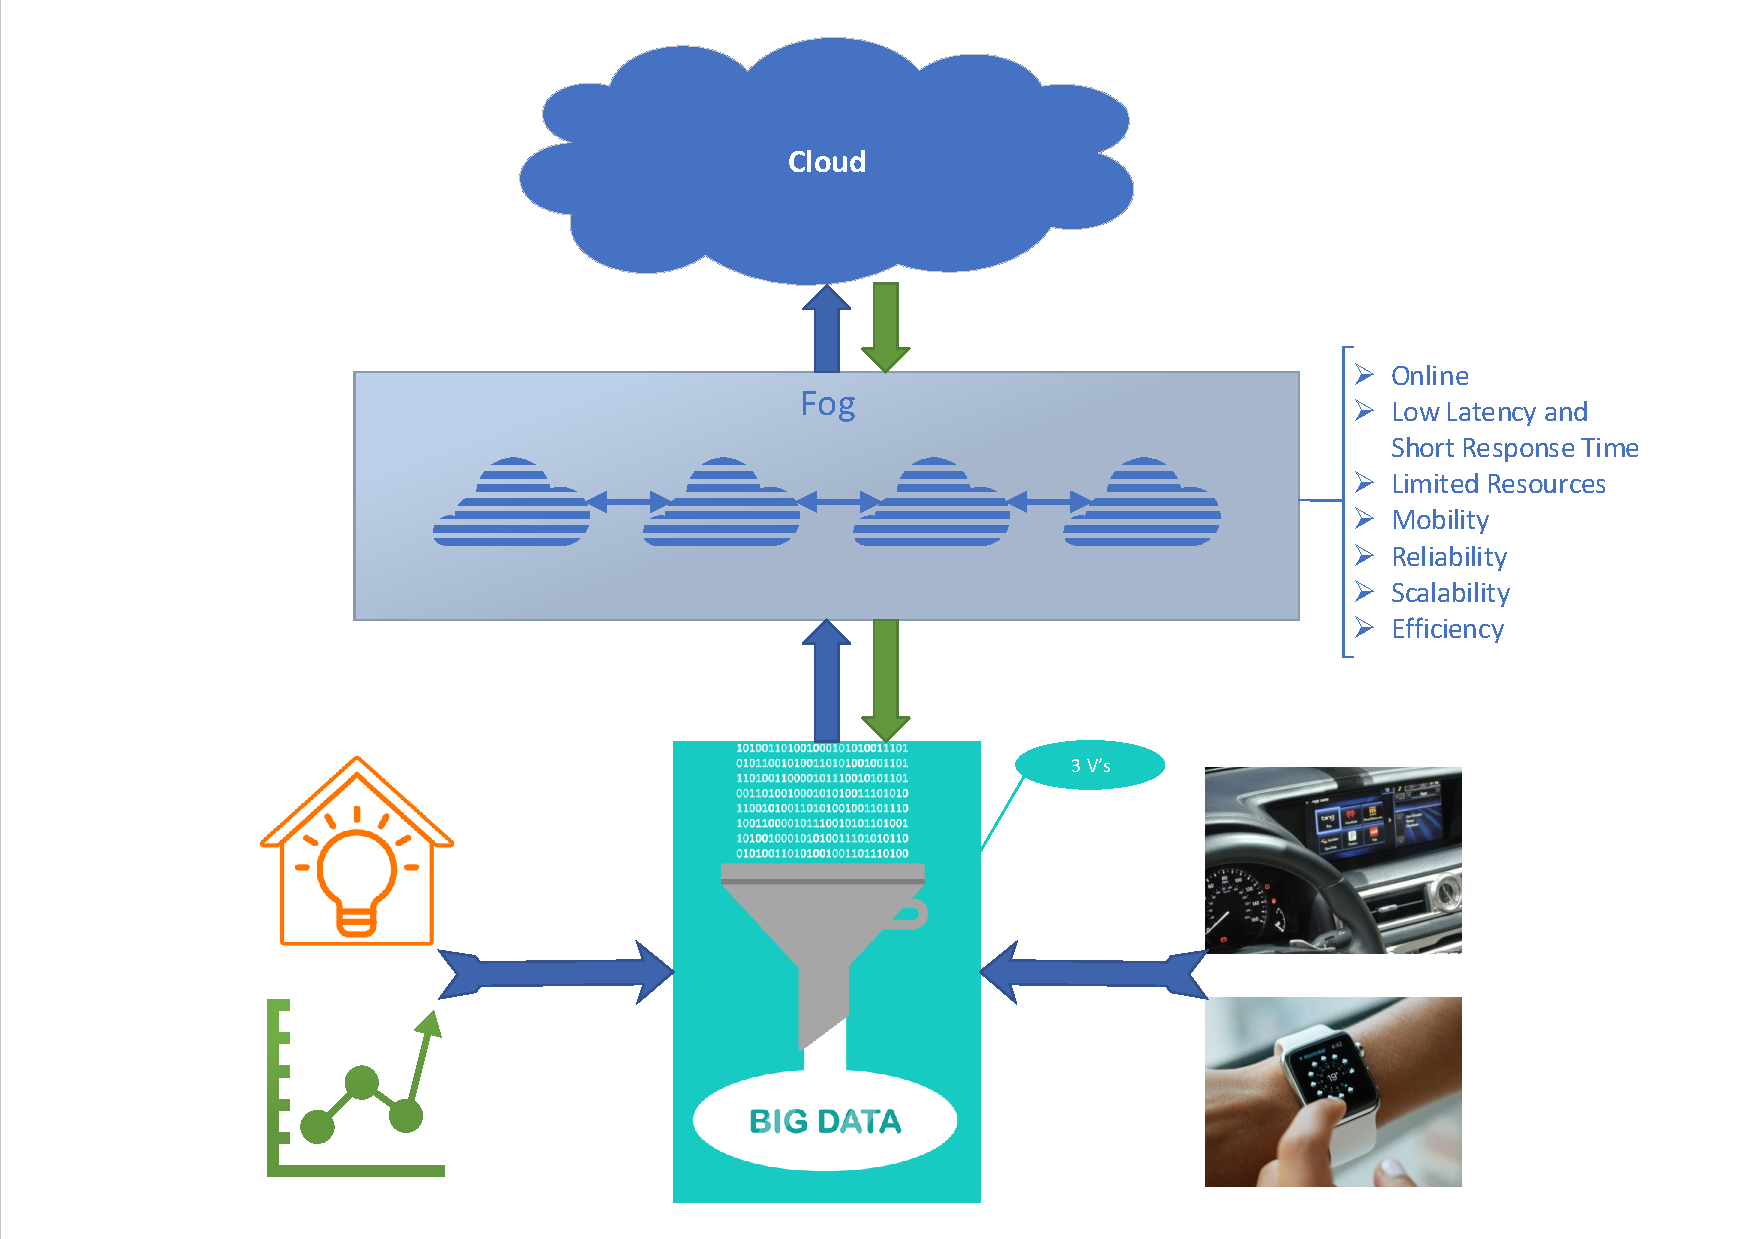
\includegraphics[width=0.4\textwidth]{figs/Data_Stream_Processing_in_Fog_Computing.pdf}
    \caption{A Fog Computing environment.}
  \end{figure}

% It is worth mentioning that, FC is sometimes referred to as ``Edge Computing'' in the literature (e.g.\,\cite{Shi2016,GarciaLopez2015}). Certain surveys, on the other hand, treat the two as separate paradigms by considering FC as a generalization of Edge Computing, with Edge Computing representing a set of network devices (including the end devices) not necessarily interacting with the cloud\,\cite{Mahmud2018}. For the sake of clarity, we will use ``FC'' to refer to the paradigm in the focus of this project, as suggested by\,\cite{cisco2012} and\,\cite{Mahmud2018}.

\subsection{Problem Specification}
We consider the healthcare application of early detection of epilepsy seizures using EEG timeseries data, because such healthcare applications require close to real-time response times.

Our goal was to achieve less network congestion between the Fog and Cloud layers as well as higher response times for the EEG sensors. More specifically, we aim for a balanced tradeoff between fast and light-weight --- even though less accurate --- computations on the IoT side, and more accurate classifications but with higher latency on the cloud side.\footnote{\emph{A note on the revision of the first two sections}: These sections have been mildly revised to \begin{enumerate*}[label=\arabic*)]
    \item more accurately reflect the actual implementation of the project, and the materials --- including the dataset used --- and,
    \item incorporate the professor's helpful comments from the project proposal.
  \end{enumerate*}}

\subsection{Related Work}
FC in general as well as different applications requiring real-time response times have been considered before. For example, Tang \etal\cite{Tang:2015} implemented a hierarchical FC architecture for anomaly detection of pipe leakage in smart cities. We were inspired by the work of Diab Abdulgalil \etal\cite{DiabAbdulgalil2018}, where they propose a FC architecture with SVM classification at the edge, and deep convolutional networks in the cloud. To the best of our knowledge, and to the date of this writing, this has been the only work which considered FC for efficient epilepsy seizures detection.

%%% Materials and Methods %%%%%%%%%%%%%%%%%%%%%%%%%%%%%%%%%%%%%%%%%%%%%%%%

 \section{Materials and Methods}\label{materials}

 \subsection{Dataset}
 Andrzejak \etal\cite{PhysRevE.64.061907}\footnote{\url{http://epileptologie-bonn.de/cms/front_content.php?idcat=193&lang=3&changelang=3}} provide a dataset of \(500\) individuals, each with \(4097\) data points for \(23.5\) seconds. This dataset is further reshaped and shuffled to \(23 \times 500 = 11500\) records, where each record contains \(178\) data points (features) for \(1\) second by Qiuyi and Fokoue on UCI Machine Learning Repository \cite{UCIDataset}. Each record of this dataset is labeled with one of 5 classes, with one class being the seizure state. Since our goal was predicting the seizures, we further restructured this dataset into \texttt{(time,value)} tuples, and considered the seizure class of consecutive \(178\) tuples as positive, and all the groups tuples belonging to other classes as negative. This resulted in \(11500 \times 178 = 2\,047\,000\) tuples, which would be simulated as a stream of data generated by an EEG sensor. The final breakdown of the dataset is shown in table~\ref{tab.dataset}.

 \begin{table}\label{tab.dataset}
    \centering
    \caption{The breakdown of the EEG timeseries dataset used.}
    \addfontfeatures{Numbers={Lining,Tabular}}
    {\begin{tabular}{@{} lrrr @{}}
      \toprule
       & Total & Positive & Negative\\
      \midrule
      Training & 7\,000 & 1\,392 & 5\,608\\
      Test & 4\,500& 908 & 3\,592\\
      \addlinespace
      Total & 11\,500 & 2\,300 & 9\,200\\
      \bottomrule
    \end{tabular}}
  \end{table}

 \subsection{Project Structure}
 We will consider a three-tier infrastructure for our FC implementation, as described below:

 \begin{enumerate}
     \item \textbf{The IoT devices/sensors:} This layer consists of the IoT data generators/producers/sensors. Such devices generate large volumes of data in a small time-frame; however, they usually lack the required processing power, storage, and energy to process this data. They may also expect a response from the higher layers depending on the event inferred from their produced data, for example, in case of a gas/pipe leak sensor.
     
     Several IoT hubs and data stream processing frameworks exist, such as Apache Kafka\footnote{\url{https://kafka.apache.org/}}, IBM Watson Internet of Things (IoT)\footnote{\url{https://www.ibm.com/internet-of-things}}, Microsoft Azure IoT Platform\footnote{\url{https://azure.microsoft.com/en-us/overview/iot/}}, etc.

     \item \textbf{The Fog layer:} The Fog layer is the intermediate layer between the end devices and the Cloud. Its job is to perform any preliminary analytics on the data, in order to both prevent the whole raw data travel to the Cloud, and to infer any fast responses required by the IoT devices in the lower layer based on the mentioned analysis. The Fog layer may also serve as a resource provisioning coordinator in some applications.
     
     At the time of this writing, the only existing framework dedicated to Fog/Edge Computing is Apache Edgent\footnote{\url{http://edgent.apache.org/}}, which is currently in a beta state.

     \item \textbf{The Cloud:} The Fog sends the results of its analyses to the Cloud for further analysis and aggregation. The Cloud may also serve as a coordinator for the bottom two layers, and/or it may send required responses or information to the IoT applications.
     
     As the Cloud services have been offered since the 2000s, there is a large number of options, both commercial and open-source. Examples include IBM Bluemix\footnote{\url{https://www.ibm.com/cloud/}}, Microsoft Azure\footnote{\url{https://azure.microsoft.com/}}, Amazon Web Services (AWS)\footnote{\url{https://aws.amazon.com/}}, and Apache Cloudstack\footnote{\url{https://cloudstack.apache.org/}}.

     Our top preference is the open-source solution --- Apache Cloudstack, while we may consider educational services of the other Cloud providers depending on the risks faced in the course of the development of the project.
 \end{enumerate}

 \subsection{Project Phases}
 We aim to proceed through the following phases for our project. Details are subject to change due to our inexperience with the FC infrastructure. Nevertheless, we believe that we will achieve the following by the end of the project deadline:
 
 \begin{itemize}
     \item We plan to develop a functional implementation of the layers described in the previous section in separation first. Since our ultimate goal is to connect each layer functionally, we will choose from the available technologies and frameworks those that we deem will best suit to this end. This phase will also include a good deal of research and experimentation with the available tools and frameworks. Meanwhile, we will also research and define an application use-case to test with our framework. The choice of the application must be approved by the supervisor of the course.
     \item For the next step, we will connect the three layers with their available APIs, and set up a fully-functioning prototype. This phase will also include part of the debugging of the infrastructure.
     \item We will implement our application use-case on the developed infrastructure. We plan to analyze the data generated by the IoT devices in the first layer, both on the Fog layer and the Cloud layer. Preferably, the two analyses will be such that the one in the Fog layer is advantageous to the Cloud. For example, we may implement data pre-processing in this layer. The certain types of analyses performed will be both determined by the specific use-case that we come up with, as will as be one mentioned during the lectures (e.g. Random Forests) as required by the project description.
     \item Finally, we plan to analyze the process, aggregate the results, discuss the challenges and future works, and compile the project report containing all said deliverables.
 \end{itemize}

 \clearpage
\bibliographystyle{plain}
\bibliography{refs}

\end{document}